\section{Force of Infection}\label{sr.foi}
This section presents supplementary results regarding
force of infection equations and assumptions.
%===================================================================================================
\subsection{Proof that $B_{\wph} \ge B_{\bph}$}\label{sr.foi.proof}
In \sref{foi.prior.bhom}, we claimed that
the per-partnership probability of transmission $B$ is larger for
within- \vs between-partnership heterogeneity
--- $B_{\wph} \ge B_{\bph}$, from \eqrefs{eq:B.wph}{eq:B.bph}, respectively ---
given the same set of transmission modifiers $R_f, \alpha_f$.
Here is a proof of that claim:
\begin{equation}
  \begin{aligned}
    B_{\wph} &\ge B_{\bph} \\
    1 - \prod_f {(1 - \beta_f)}^{A\alpha_f} &\ge 1 - \sum_f \alpha_f {(1 - \beta_f)}^{A}
  \end{aligned}
\end{equation}
Let $x_f = {(1 - \beta_f)}^A$; then
\begin{equation}\label{eq:AM-GM}
  \prod_f {x_f}^{\alpha_f} \le \sum_f \alpha_f x_f
\end{equation}
Since $\sum_f \alpha_f = 1$ and $\alpha_f \in [0,1]$ are effectively weights,
\eqref{eq:AM-GM} is the weighted arithmetic mean--geometric mean (AM-GM) inequality \cite{Aldaz2009}.
In fact, \citet{Aldaz2009} further shows that the gap between $B_{\wph}$ and $B_{\bph}$
increases with the $\alpha_f$-weighted variance in ${\beta_f}^{\frac12}$
(although the increase is not exact),
which supports the results of \sref{foi.exp.xph} mathematically.
\par
Using Jensen's inequality \cite{Jensen1906} we can also show that
the approach in \cite{Kerr2015} (and others)
to aggregate heterogeneity by HIV infection stage first
produces an intermediate per-partnership probability $B_{\xph}$:%
\footnote{\hreftt{math.stackexchange.com/questions/4660409}}
\begin{equation}
  B_{\wph} \ge B_{\xph} \ge B_{\bph},
  \qquad B_{\xph} = 1 - {(1 - \sum_f \alpha_f \beta_f)}^{A}
\end{equation}
%===================================================================================================
\subsection{Illustrative Scenario}\label{sr.foi.toy}
Consider the moment of one transmission event
in a population of 16 monogamous partnerships, with 25\% infection prevalence
and random mixing by infection status (Figure~\ref{fig:foi.toy.pair}).
Initially, infection prevalence is equal among partners of
susceptible $S$ and infectious $I$ individuals: 6/24 and 2/8, respectively.
Immediately after transmission,
prevalence decreases to 5/23 among partners of $S$ but increases to 4/9 among partners of $I$,
decreasing the population-level transmission risk.
Next, three events are possible:
\begin{enumerate}
  \item[(a)] \label{toy.e.t}
  another transmission occurs among the remaining $S$-$I$ partnerships,
  yielding 4/22 prevalence among partners of $S$, and 6/10 among partners of $I$;
  population-level transmission risk decreases further
  \item[(b)] \label{toy.e.p}
  the partnership from the original transmission ends,
  and both individuals form new partnerships (assumed at random),
  yielding, on average, 9/32 prevalence among partners of both $S$ and $I$;
  population-level transmission risk increases \emph{above} the initial level ($9/32 > 6/24$)
  \item[(c)] \label{toy.e.q}
  any other partnership ends,
  and both individuals form new partnerships (assumed at random);
  infection prevalence among $S$ and $I$, and population-level transmission risk
  all remain unchanged, on average
\end{enumerate}
Prior compartmental models have effectively assumed that
event (b) always occurs before (a)
--- \ie the ``instantaneous partnership assumption''.
This assumption is reflected in Figure~\ref{fig:foi.toy.freq},
where the frequentist approximation does not explicitly model any individual partnerships.
This assumption is evidently worse for longer partnerships.
\begin{figure}
  \begin{subfigure}{.5\linewidth}
    \centering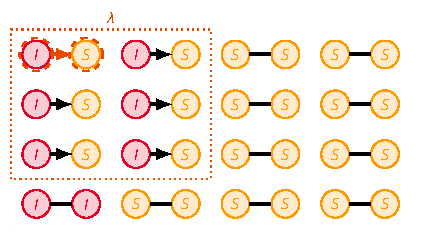
\includegraphics[scale=1]{foi.toy.pair}
    \caption{Pair-wise reality}
    \label{fig:foi.toy.pair}
  \end{subfigure}%
  \begin{subfigure}{.5\linewidth}
    \centering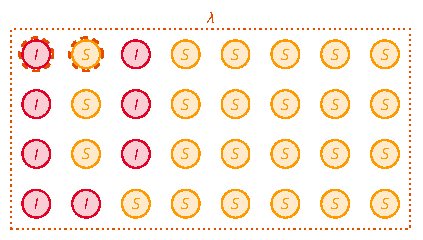
\includegraphics[scale=1]{foi.toy.freq}
    \caption{Frequentist approximation}
    \label{fig:foi.toy.freq}
  \end{subfigure}
  \caption{Comparison of pair-based reality and frequentist approximation
    for a population of 16 pairs with 25\% infection prevalence,
    at the moment of one transmission event}
  \label{fig:foi.toy}
  \floatfoot{
    $S$: susceptible; $I$: infectious; $\lambda$: force of infection;
    dashed circles: individuals involved in transmission event.}
\end{figure}
%===================================================================================================
\subsection{Calibration}\label{sr.foi.cal}
% TODO: (!)
\begin{figure}
  \centering\includegraphics[scale=1]{ll.hist.foi}
  \caption{}
  \label{fig:ll.hist.foi}
  \floatfoot{\fffoi.}
\end{figure}
\begin{figure}
  \centering\includegraphics[width=\linewidth]{post.distr.foi}
  \caption{Posterior distributions of calibrated model parameters,
    under different force of infection approaches (colours)}
  \label{fig:post.distr.foi}
  \floatfoot{\ffpar; \fffoi; \ffpost;
    \ffast{QN rank score test \cite{Kruskal1952} for comparing distributions}}
\end{figure}
This section illustrates the results of model calibration
under the four force of infection approaches explored in \sref{foi.exp.model}:
Effective Partnerships Reduction (\epa),
Instantaneous Rate-Duration (\ird),
Instantaneous Rate-1-Year (\iry), and
Instantaneous Proportion-1-Year (\ipy).
Figures~\ref{fig:fit.prev.foi}--\ref{fig:fit.inc1v2.foi} illustrate the modelled HIV
prevalence, prevalence ratios, incidence, and incidence ratios,
plus associated calibration targets, for each approach.
Qualitative differences between approaches appear to be minimal,
except for lower incidence among FSW in Figure~\ref{fig:fit.inc.foi-py},
as expected (see \sref{foi.exp.mod.dyn}).
\par
\foreach \vf/\var/\vlab in {%
  1/prev/prevalence,%
  1/prev1v2/prevalence ratios between selected risk groups,%
  1/inc/incidence,%
  .6/inc1v2/incidence ratios between selected risk groups}{
  \begin{figure}[h]
    \subcapoverlap\centering
    \foreach \foi in {base,foi-rd,foi-ry,foi-py}{
      \begin{subfigure}{\vf\linewidth}
        \centerline{\includegraphics[scale=\fitscale]{fit.\var.\foi.all}}
        \caption{\raggedright}
        \label{fig:fit.\var.\foi}
      \end{subfigure}\\}
    \caption{Modelled HIV \vlab and associated calibration targets
      under different force of infection approaches}
    \label{fig:fit.\var.foi}
    \floatfoot{Approaches:
      \foreach \foi/\flab in {base/\epa,foi-rd/\ird,foi-ry/\iry,foi-py/\ipy}{
        \sfref{fig:fit.\var.\foi}: \flab;}
      \fffoi; \fffit; \ffribbon; \ffpbar.}
  \end{figure}}
%===================================================================================================
\subsection{Distributions of Infections}\label{sr.foi.exp}

\begin{figure}
  \includegraphics[width=\linewidth]{foi.wiw.part}
  \caption{Proportions of modelled yearly HIV infections
    transmitted via different partnership types in Eswatini
    estimated under different force of infection approaches (horizontal facets)
    with equal \vs approach-specific parameters (vertical facets)}
  \label{fig:foi.wiw.part}
  \floatfoot{\fffoi; \ffwiw.}
\end{figure}
